%!TEX root = ../template.tex
%%%%%%%%%%%%%%%%%%%%%%%%%%%%%%%%%%%%%%%%%%%%%%%%%%%%%%%%%%%%%%%%%%%%
%% chapter3.tex
%% NOVA thesis document file
%%
%% Chapter with a short latex tutorial and examples
%%%%%%%%%%%%%%%%%%%%%%%%%%%%%%%%%%%%%%%%%%%%%%%%%%%%%%%%%%%%%%%%%%%%

\typeout{NT FILE chapter3.tex}%

\makeatletter
\newcommand{\ntifpkgloaded}{%
	\@ifpackageloaded%
}
\makeatother

\chapter{Algoritmi esatti per il \gls{TSP}} \label{chapt:3}

Questo capitolo fornisce un esame approfondito degli algoritmi esatti per risolvere il \gls{TSP}, incorporando pseudocodice dettagliato per chiarire i principi operativi di ciascun metodo. Attraverso questi algoritmi, esploriamo il panorama computazionale della ricerca di soluzioni ottimali al \gls{TSP}.

\section{Panoramica degli Algoritmi Esatti}

Gli algoritmi esatti per il \gls{TSP} sono caratterizzati dalla loro capacità di trovare invariabilmente la soluzione ottimale, sebbene con costi computazionali che possono diventare proibitivi man mano che il numero di città aumenta. Questi algoritmi servono come base teorica e pratica per comprendere i limiti della risoluzione computazionale del \gls{TSP}.

\subsection{Metodo a Brute-Force}

Il metodo a forza bruta esamina sistematicamente ogni possibile tour per identificare quello con la distanza totale più bassa. Nonostante la sua semplicità, la crescita esponenziale dei calcoli lo rende impraticabile per grandi istanze.

\begin{algorithm}
	\caption{TSP Brute Force}\label{bruteforce}
	\begin{algorithmic}[1]
		\Procedure{BruteForceTSP}{$cities$}
		\State $min\_distance \gets \infty$
		\State $min\_tour \gets \emptyset$
		\ForAll{tours $t$ of $cities$}
		\State $distance \gets$ \textsc{TourDistance}($t$)
		\If{$distance < min\_distance$}
		\State $min\_distance \gets distance$
		\State $min\_tour \gets t$
		\EndIf
		\EndFor
		\State \Return $min\_tour$
		\EndProcedure
	\end{algorithmic}
\end{algorithm}

La complessità computazionale di questo metodo è $O(n!)$, che riflette il numero fattoriale di tour che devono essere valutati.

\subsection{Algoritmo di Bellman-Held-Karp}

L'algoritmo di Bellman-Held-Karp rappresenta un significativo avanzamento nelle soluzioni esatte del \gls{TSP} sfruttando la programmazione dinamica per ridurre l'onere computazionale. Questo approccio calcola il percorso più breve dividendo il problema in sottoproblemi più piccoli e memorizzando i risultati di questi sottoproblemi per evitare calcoli ridondanti.

\begin{algorithm}
	\caption{Algoritmo di Bellman-Held-Karp}\label{bellmanheldkarp}
	\begin{algorithmic}[1]
		\Procedure{BellmanHeldKarp}{$cities$}
		\State Crea una tabella $distances$ per memorizzare i percorsi più brevi
		\State Inizializza tutte le voci in $distances$ a $\infty$
		\State $distances[1][\{1\}] \gets 0$ \Comment{Città di partenza}
		\For{$m = 2$ to $|cities|$}
		\ForAll{sottoinsiemi $S$ di $cities$ di dimensione $m$ contenenti 1}
		\ForAll{$j \in S, j \neq 1$}
		\State $distances[j][S] \gets \min_{k \neq j, k \in S} (distances[k][S\setminus\{j\}] + distance(k, j))$
		\EndFor
		\EndFor
		\EndFor
		\State \Return $\min_{j}(distances[j][cities] + distance(j, 1))$
		\EndProcedure
	\end{algorithmic}
\end{algorithm}

L'algoritmo di Bellman-Held-Karp opera con una complessità temporale di $O(n^2 \cdot 2^n)$~\ref{fig:agl_complexity}, rendendolo significativamente più efficiente del metodo a forza bruta per istanze di problema di dimensioni moderate. Tuttavia, la componente esponenziale della sua complessità limita ancora la sua applicabilità pratica a istanze relativamente piccole di \gls{TSP}.

\subsubsection{Branch and Bound}

Branch and Bound (\gls{BnB}) è una tecnica algoritmica generale che può essere applicata a vari problemi di ottimizzazione combinatoria, incluso il \gls{TSP}. Esplora sistematicamente lo spazio delle soluzioni dividendolo in sottoinsiemi più piccoli (branching) e utilizzando limiti per eliminare i sottoinsiemi che non contengono la soluzione ottimale, riducendo così lo spazio di ricerca.

\begin{algorithm}
	\caption{\gls{BnB} per il \gls{TSP}}\label{branchbound}
	\begin{algorithmic}[1]
		\Procedure{BranchAndBoundTSP}{$cities$}
		\State Inizializza una coda di priorità $Q$ con una soluzione parziale che parte dalla prima città
		\State $min\_distance \gets \infty$
		\While{$Q$ non è vuota}
		\State Prendi la soluzione parziale con il limite inferiore più basso da $Q$
		\If{rappresenta un tour completo}
		\If{il suo costo è inferiore a $min\_distance$}
		\State Aggiorna $min\_distance$ e registra il tour
		\EndIf
		\Else
		\State Dividi aggiungendo una città alla soluzione parziale
		\State Calcola i limiti per le nuove soluzioni parziali
		\State Aggiungi le nuove soluzioni parziali a $Q$
		\EndIf
		\EndWhile
		\State \Return $min\_distance$
		\EndProcedure
	\end{algorithmic}
\end{algorithm}

L'efficienza di \gls{BnB} per il \gls{TSP} dipende in modo significativo dalla funzione di limite utilizzata per stimare il limite inferiore delle soluzioni parziali. Un limite efficace può portare a riduzioni sostanziali dello spazio di ricerca, consentendo all'algoritmo di trovare la soluzione ottimale più rapidamente rispetto ai metodi di ricerca esaustiva. Tuttavia, la sua complessità temporale peggiore rimane $O(n!)$~\ref{fig:agl_complexity}, il che significa che per istanze molto grandi del problema, anche questo approccio sofisticato potrebbe non essere pratico.

\section{Analisi degli Algoritmi Esatti}

\subsection{Fattibilità Computazionale}

Gli algoritmi esatti per il \gls{TSP}, come il metodo a forza bruta, la programmazione dinamica e l'algoritmo di Held-Karp, offrono garanzie teoriche per trovare il tour ottimale. Tuttavia, la loro fattibilità computazionale è notevolmente compromessa all'aumentare del numero di città. Il tasso di crescita fattoriale della complessità del metodo a forza bruta e il tasso di crescita esponenziale della complessità della programmazione dinamica e di Held-Karp limitano la loro applicazione pratica a istanze relativamente piccole del \gls{TSP}.

%\begin{center}
\begin{figure}[h]
	\caption{Complessità degli Algoritmi Esatti}
	\label{fig:agl_complexity}
	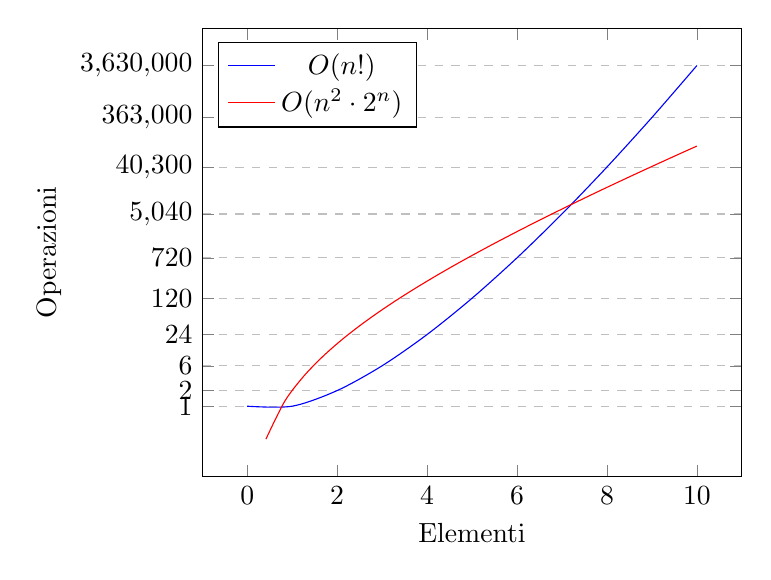
\begin{tikzpicture}
		\begin{semilogyaxis}[
				xlabel={Elementi},
				ylabel={Operazioni},
				domain=0:10,
				ytick={0,1,2,6,24,120,720,5040,40320,362880,3628800},
				log ticks with fixed point,
				legend pos=north west,
				ymajorgrids=true,
				grid style=dashed,
			]
			\addplot+[mark=none,smooth] coordinates {
					(0,1) (1,1) (2,2) (3,6) (4,24) (5,120) (6,720) (7,5040)
					(8,40320) (9,362880) (10,3628800)
				};
			\addlegendentry{$O(n!)$}

			\addplot+[mark=none,smooth] expression {x^2 * 2^x};
			\addlegendentry{$O(n^2 \cdot 2^n)$}

		\end{semilogyaxis}
	\end{tikzpicture}
\end{figure}
%\end{center}

\subsection{Vantaggi e Svantaggi}
Riassumendo:

\textbf{Vantaggi:}
\begin{itemize}
	\item Garanzia di trovare una soluzione ottimale.
	\item Forniscono un benchmark per valutare le prestazioni di algoritmi euristici e meteuristici.
\end{itemize}

\textbf{Svantaggi:}
\begin{itemize}
	\item Complessità temporale esponenziale che li rende impraticabili per grandi istanze.
	\item Significative risorse computazionali richieste anche per problemi di dimensioni moderate.
	\item La programmazione dinamica e Held-Karp, pur essendo più efficienti del metodo a forza bruta, affrontano ancora limitazioni a causa della loro complessità spaziale e della necessità di un calcolo estensivo.
\end{itemize}

L'esplorazione degli algoritmi esatti getta le basi per comprendere le complessità computazionali intrinseche del \gls{TSP}. Sebbene la loro applicazione pratica sia limitata dalle loro esigenze computazionali, rimangono cruciali per l'analisi teorica e per preparare il terreno per le tecniche risolutive alternative discusse nei capitoli successivi.

